\begin{center}
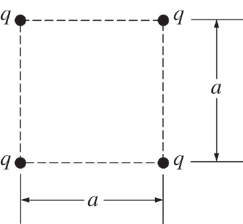
\includegraphics[scale=0.5]{images/img-010-031.png}
\end{center}

% Multiple Choice Question 34
\begin{questions}\setcounter{question}{33}\question
Four identical point charges $q$ are fixed at the corners of a square with sides of length $a$, as shown above. The potential at the center of the square due to these charges is

\begin{oneparchoices}
\choice zero
\choice $\dfrac{1}{4 \pi \epsilon_{0}} \dfrac{q}{\sqrt{2} a} $
\choice $\dfrac{1}{4 \pi \epsilon_{0}} \dfrac{q}{a}$
\choice $\dfrac{1}{4 \pi \epsilon_{0}} \dfrac{4 q}{a}$
\choice $\dfrac{1}{4 \pi \epsilon_{0}} \dfrac{4 \sqrt{2} q}{a}$
\end{oneparchoices}\end{questions}

